\chapter{背景・関連研究}
\label{cha:background}

本章では，本研究の背景となる
皮膚表面下散乱および関連研究について整理する。
まず，表面下散乱の基本的な考え方と，
それを記述するBSSRDFについて概説する。
次に，皮膚を対象とした代表的な表面下散乱モデルを紹介する。
さらに，毛髪や髭の表現に関する既存研究について述べ，
最後に本研究の位置づけを明確にする。

\section{表面下散乱とBSSRDF}
物体表面における反射現象は，
一般に双方向反射率分布関数
(Bidirectional Reflectance Distribution Function: BRDF)
によって記述される。
BRDF は，
入射光と出射光が同一の表面点で相互作用することを前提としており，
金属やプラスチックなどの不透明な物体に対して有効である。

一方で，人間の皮膚や大理石，ワックスなどの半透明物体では，
光が表面から内部に侵入し，
内部で散乱した後，
異なる位置から出射する現象が観測される。
このような表面下散乱を扱うため，
双方向表面下散乱反射率分布関数
(Bidirectional Surface Scattering Reflectance Distribution Function: BSSRDF)
が導入された。
\begin{figure}[tb]
  \centering
  \subfloat[BRDF]{
    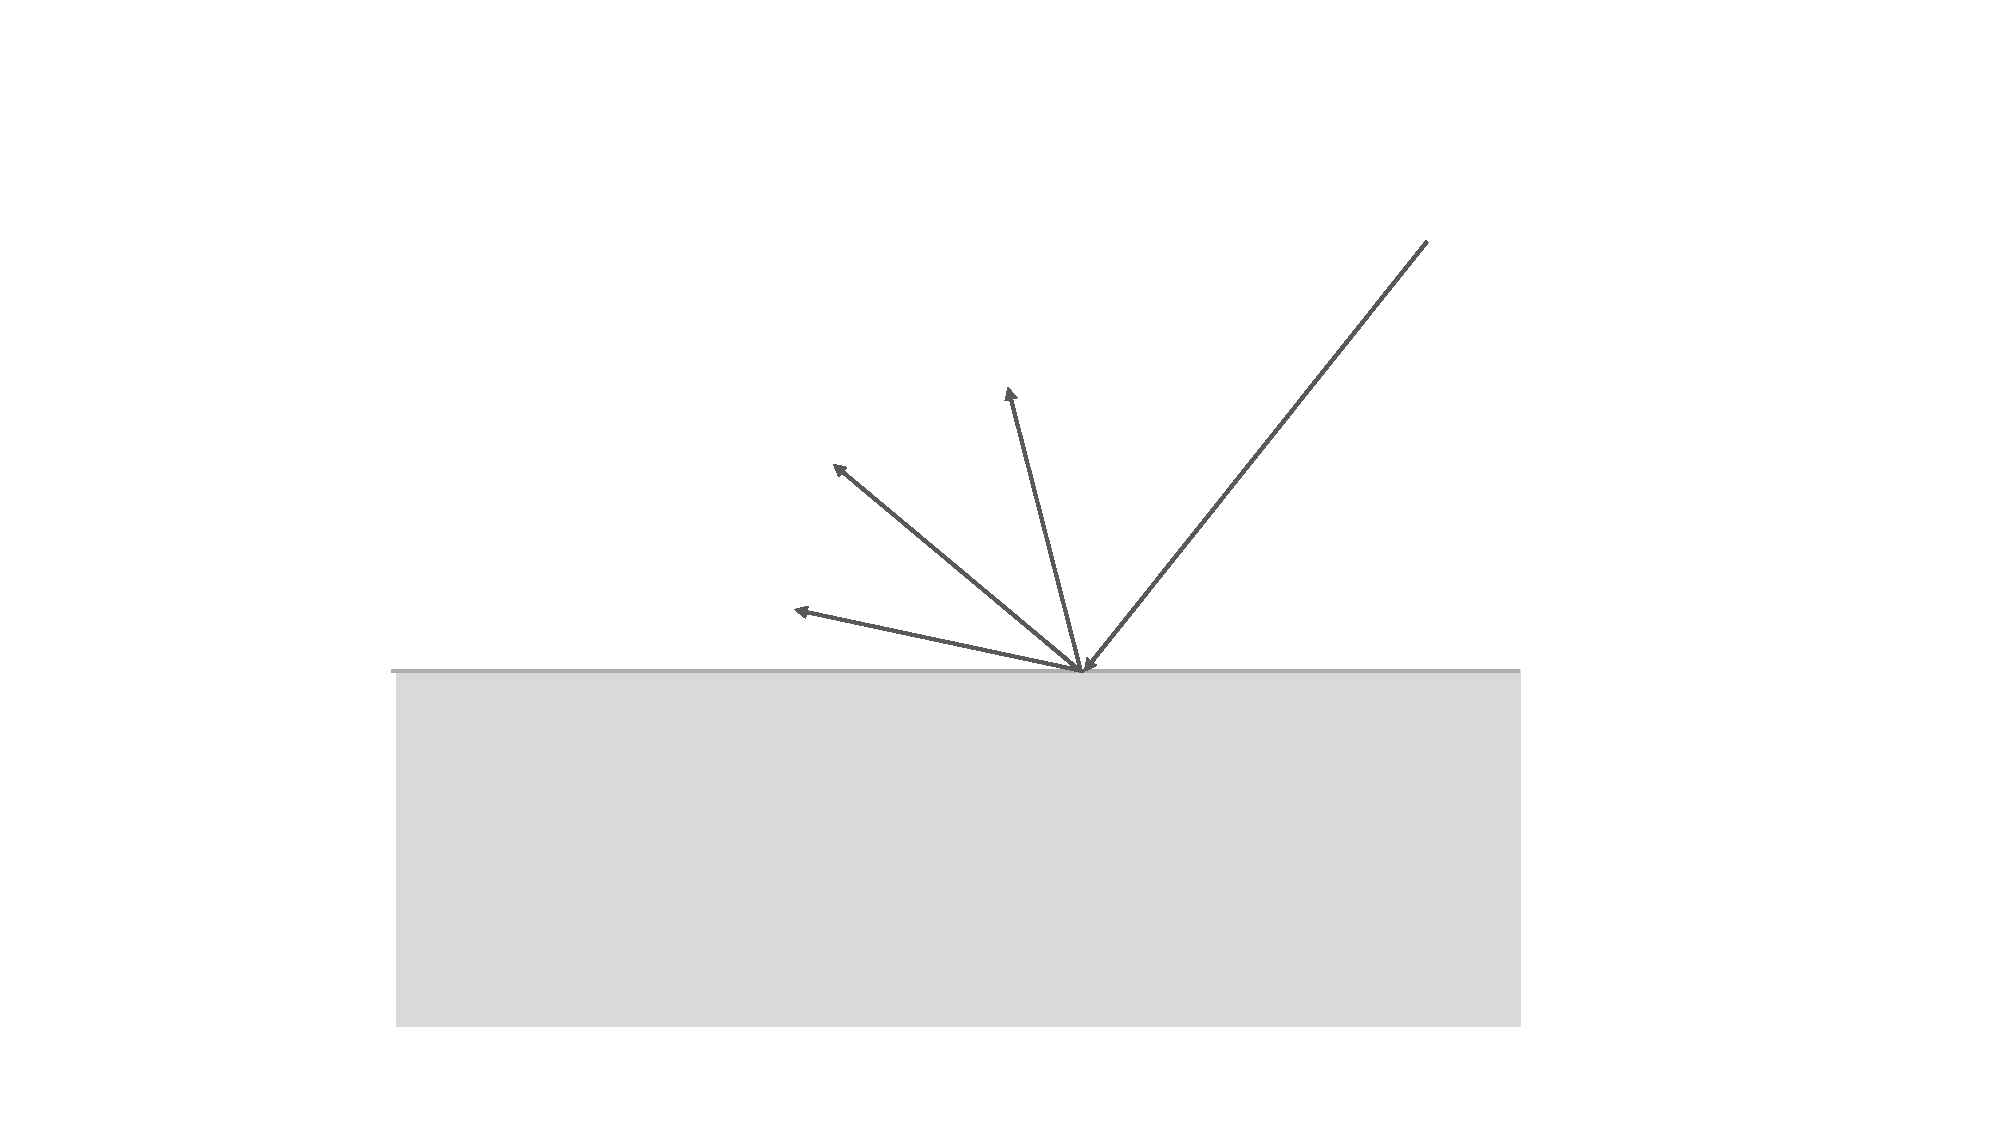
\includegraphics[width=0.46\linewidth]{figs/BRDF.pdf}
  }
  \hspace{0.04\linewidth}
  \subfloat[BSSRDF]{
    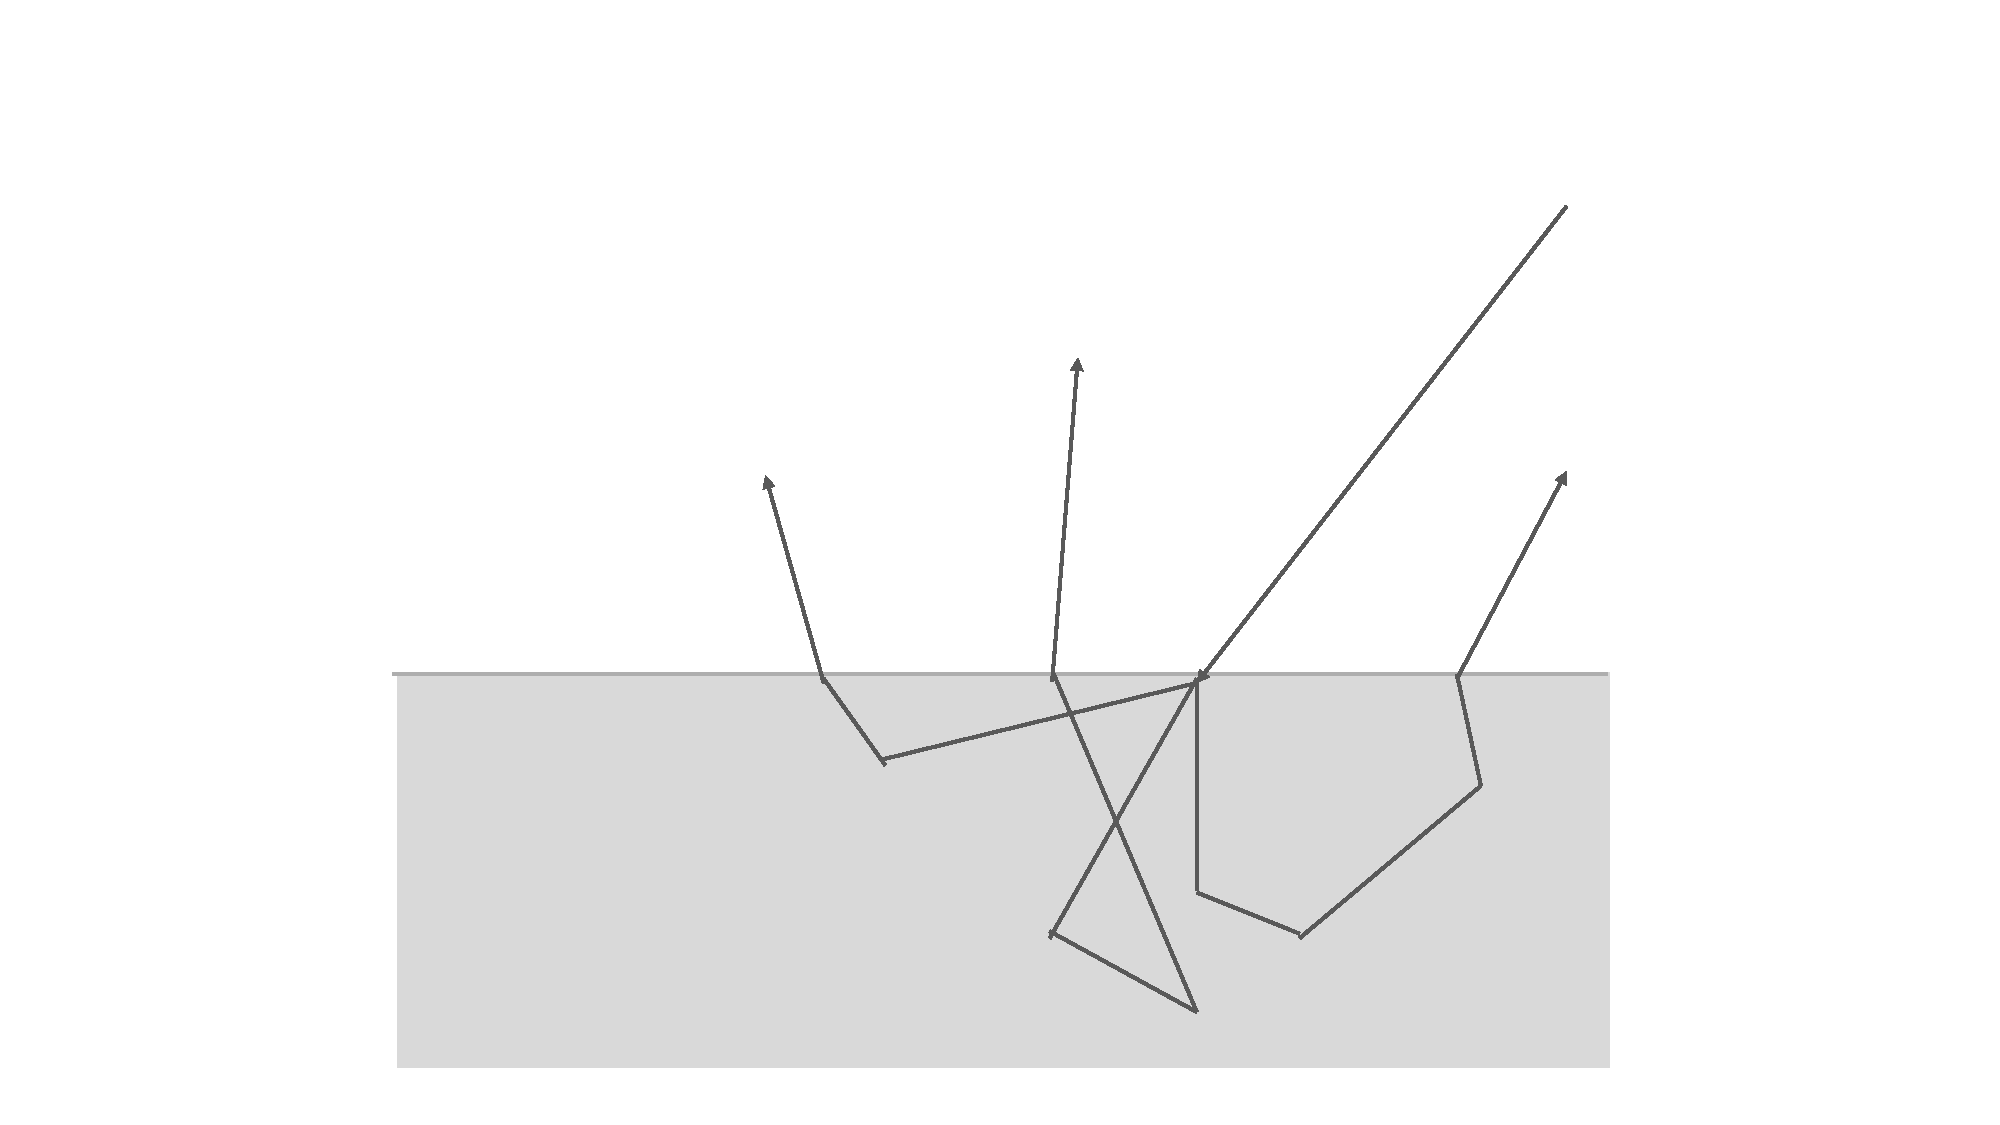
\includegraphics[width=0.46\linewidth]{figs/BSSRDF.pdf}
  }
  \caption{BRDF と BSSRDF による光輸送モデルの違いの概念図（文献\cite{Jensen2001Dipole}を参考に作成）。}
  \label{fig:brdf_bssrdf}
\end{figure}
\section{皮膚の表面下散乱モデル}
皮膚は，表皮，真皮，皮下組織といった
複数の層から構成される多層構造を持ち，
各層で異なる吸収・散乱特性を示す。
これらを厳密に扱うためには，
放射輸送方程式を解く必要があるが，
計算コストが高いため，
実用的なレンダリングでは近似モデルが用いられる。

皮膚表面下散乱モデルの代表的な研究として，
Donner と Jensen による研究
\cite{Donner2006Spectral}
が挙げられる。
この研究では，
皮膚内部での光の散乱を
スペクトル領域で扱うBSSRDFモデルが提案されており，
皮膚に特有な色変化や透明感を
高い精度で再現できることが示されている。
同手法は拡散近似に基づいており，
計算効率と写実性の両立を実現した点で，
皮膚表現に関する多くの後続研究の基盤となっている。

\begin{figure}[tb]
  \centering
  
\includegraphics[width=0.8\linewidth]{figs/chot_1.jpg}
  \caption{人間の皮膚における多層構造と光輸送の概念図。
皮膚は表皮，真皮，皮下組織など
複数の層から構成されており，
各層で光の吸収および散乱特性が異なる。
このような層構造を考慮することで，
皮膚表面下散乱のより現実的な表現が可能となる。}
  \label{fig:skin_layers}
\end{figure}
さらに，
Weyrich らによる研究
\cite{Weyrich2008Layered}
では，
皮膚を多層構造かつ空間的に不均質な媒質として扱う
反射モデルが提案されている。
この研究では，
実測データに基づいて皮膚の層構造を取得し，
層ごとに異なる光学特性を持たせることで，
より現実的な皮膚表現を実現している。

これらの研究は，
皮膚が一様な媒質ではなく，
層構造や空間的な不均質性を持つことを示しており，
皮膚表面下散乱モデルの高度化に大きく貢献している。

\section{毛髪・髭表現に関する研究}
毛髪表現に関する研究は，
主に頭髪を対象として発展してきた。
毛髪一本一本を幾何的に表現し，
異方的な反射モデルを適用することで，
写実的な見えを再現する手法が数多く提案されている。

一方で，
顔に存在する髭は，
頭髪と比較して短く，
高密度に分布するという特徴を持つ。
そのため，
毛髪一本単位での厳密な表現は，
計算コストの観点から
実用的でない場合が多い。

多くの皮膚表面下散乱モデルでは，
皮膚内部の光学特性に焦点が当てられており，
皮膚表面付近に局所的に分布する構造物，
例えば髭のような毛髪要素については，
明示的には扱われていない。
その結果，
髭が存在する領域においても
皮膚のみの場合と同様の散乱特性が適用され，
見えの違いが十分に表現されないという問題がある。

\section{本研究の位置づけ}
以上のように，
皮膚表面下散乱に関する研究は数多く存在する一方で，
髭のような局所的な構造物が
皮膚表面下散乱に与える影響を，
簡潔かつ実用的に取り込む手法は
十分に検討されていない。

本研究は，
Donner と Jensen による
皮膚表面下散乱モデルや，
Weyrich らによる
多層・不均質皮膚モデルを基盤としつつ，
髭という局所的不均質性を
髭密度という形で表現し，
皮膚表面下散乱モデルに組み込む点に特徴がある。

毛髪一本単位の厳密なモデル化を行うのではなく，
髭の分布を密度マップとして集約することで，
計算効率を保ちながら，
髭の存在による見えの変化を
連続的に表現することを目指す。

次章では，
本研究で提案する
髭密度を考慮した皮膚表面下散乱モデルについて
詳しく説明する。












